% The Introduction should frame the scientific issues that motivate the study. It should briefly indicate the study's objectives and provide enough background information to clarify why the study was undertaken and what hypotheses were tested. An overview of the key publications in the field is essential.
\chapter{Introduction}
\label{sec:introduction}

% - Free Play
Humans are capable of exploring and learning about the world in a self-supervised free-form manner with no explicit predefined goal.
This \emph{free play} has been established as a crucial component for the development of cognitive skills, acquisition of knowledge about the world, and adaptation to new environments \citep{exploration,chu2020play,playreview}.

% This is a process that is freely chosen, personally directed and intrinsically motivated.
% Play in humans is characterized by creativity, imagination, and a lack of extrinsic goals \citep{playmontana}.
% It has no predefined outcome and is driven by intrinsic motivation, curiosity, and the desire to explore and experiment with the environment.

% There are various aspects to play in developmental psychology, which includes construction play and expressive play .
% Creativity is evident in role play, construction activities, and other forms of imaginative play. Imagination allows children to create mental images related to their feelings, thoughts, and ideas, which they then incorporate into their play. [4]

% Playful learning is meaningful when it links new experiences - like seeing a horse in a field - to familiar ones - like the horse in a child's favourite picture book. 
% Making connections between familiar and unfamiliar stimuli guides the brain in making effortful learning easier.
% Meaningful experiences introduce novel stimuli linking to existing mental frameworks; processing these stimuli recruits networks in the brain associated with analogical thinking, memory, transfer, metacognition, creating insight, motivation and reward.


% Meaningful experiences present a blend of familiar
% and novel stimuli, initiating neural networks involved
% with novelty processing, memory, and reward seeking
% exploration that are useful in learning (Bunzeck,
% Doeller, Dolan, & Duzel, 2012). Studies demonstrate
% that familiar inputs combined with a novel reward
% can result in stronger hippocampal activity than
% familiar stimuli with familiar reward predicted
% (Bunzeck et al., 2011). 

% Lastly, some evidence tells us that the formation
% of new insights are encoded in our memories by
% activating the brain’s internal reward network
% (Kizilirmak et al., 2016). Involving the intrinsic reward
% system activates the hippocampus, which is useful
% for encoding the meaningful relationship we have
% just acquired, as well as its later retrieval (Kizilirmak
% et al., 2016).

% Taken together, discovering meaningful relationships
% in learning through play may build on various cognitive
% processes, activate the brain’s reward system, and
% strengthen the encoding of these memories. These
% can be forceful drivers of learning. It makes sense,
% then, to provide children with material that is both
% novel and familiar. We can use this approach to
% facilitate meaningful experiences for children, guiding
% them in new explorations through play, for example,
% that deepen their own relationship with the world.

% \todo{Talk more about the importance of free play.}
% \todo{Add more developmental psychology and cognitive science references about creative exploration in children and adults}
% \todo{Talk about the correlation between intelligence acquisition and free play}

% \todo{Characteristics of free play - going to previous biases towards free play}

% - Bias towards semantics in cognitive science
Free play in humans is deeply intertwined with visual perception and meaning, and our inherent preferences for visual semantics play a pivotal role in guiding our curiosity-driven exploration, i.e. we constantly seek to understand the semantics of the objects and scenes we encounter based on our prior experiences.
This is particularly apparent in children as they spend substantial time fiddling with toys, scribbling, or playing with building blocks, eventually creating patterns and structures that are meaningful to them.
In a study on free play conducted by \citet{diggs}, participants predominantly showed a preference for semantic expression in the form of regular and symmetric patterns to depict a real-world object or concept.
This suggests that humans have an intrinsic bias or motivation towards visual semantics, i.e. a propensity to explore their environments in expressive styles that manifest their previous knowledge and understanding of the world.

% \vspace{12pt}
\begin{figure}[h]
    \centering
    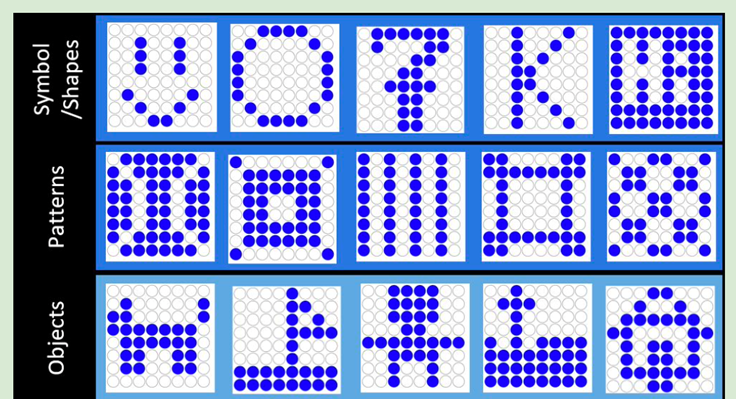
\includegraphics[width=0.7\textwidth]{images/diggs.png}
    \captionsetup{justification=centering}
    \caption[Some creations from the free-play study on humans by \cite{diggs}.]{Some creations from the free-play study on humans by \cite{diggs}.\\(Taken from the original publication.)}
    \label{fig:diggs}
\end{figure}
% \vspace{12pt}

% \todo{Find more references on this bias towards semantics in cognitive science}
% Cedric Collas and Pierre-Yves Oudeyer have some papers on this bias towards semantics in developmental psychology.

In the context of artificial intelligence, self-supervised learning has been a topic of interest for researchers in the fields of robotics and machine learning (ML), and the ability to efficiently and sufficiently explore remains a fundamental challenge.
In recent years, reinforcement learning (RL) has emerged as a powerful framework for training agents to learn complex behaviors through trial and error.
However, most RL algorithms are designed to solve specific tasks and are not well-suited for free-form exploration.
Instead, complementary formulations of novelty-based \cite{burda2018largescale,novel_explore} or uncertainty-based exploration \citep{rnd,plan_explore,disagreement} methods have been proposed to encourage agents to explore their environment in a self-supervised manner \citep{exploration_survey}. 
Yet, these methods are often unable to generate diverse and creative behaviors that are characteristic of human exploration.


% \todo{Play vs exploration}

% \todo{Comments on shaping of clip rewards near and far from the goal states}
% CLIP rewards are well-shaped around the goal state, whereas near the starting state, they are poorly shaped.

% \todo{Better segregate the different exploration methods (maybe in methods)}

% - Vision Language Models
This thesis focuses on the role of visual semantic bias in shaping these choices, proposing that our innate visual preferences act as a compass, directing our attention and interactions during free play.
Our work tries to imbue artificial agents with a visual semantics bias, akin to that in humans.
We do this by leveraging large vision language models (VLMs).
Also termed "foundational models", these deep neural networks are trained on massive generic text and image datasets using the recent advances in self-supervised learning. 
The abstractions of natural language, which reflect the semantics of the world, allow them to learn efficient representations that essentially encapsulate human visual understanding.

% - VLM Applications
VLMs are capable of successfully transferring to a diverse range of downstream applications, such as visual detection, classification, and question-answering.
However, the use of foundation models for control and embodied intelligence is relatively new and under-explored.

Pre-trained vision-language encoders, such as CLIP \citep{clip}, have been used far beyond their original scope such as image generation \citep{imagegeneration}, robot control \citep{cliport,embodied}

% In RL, pretraining has been used to improve the representations of the policy network. 
% Pretrained CLIP features have been used in various recent robotics papers to speed up control and navigation tasks.
% These features can condition the policy network [26] or can be fused throughout the visual encoder to integrate semantic information about the environment [37]. 
% The goal of these works is to improve the perception of the policy.
% Pretrained language models can also provide useful initializations for training policies to imitate offline trajectories [42, 27].
% These successes demonstrate that large pre-trained models contain prior knowledge that can be useful for RL. While the existing literature uses pre-trained embeddings directly in the agent, we instead allow the policy network to learn from scratch and only utilize pre-trained embeddings to guide exploration during training (Figure S2).
% We imagine that future work may benefit from combining both approaches.

% - VLM as Rewards
Recent work \citep{zest,negprompt,vlmrm,lamp} has shown that they can be used as effective abstractions to generate zero-shot rewards for language-guided goal-conditioned tasks.
There are also other studies on using VLMs for exploration \citep{vlmlang,vlmdistill} that use them for refining intrinsic reward signals by abstracting away pseudo-novelty. 

% - Entropy Rewards
Yet this is fundamentally different from our goal as we are specifically interested in creative semantic expression.
Moreover, the existing studies do not consider the free-form exploration paradigm that is of interest to us; they require a specific goal to be achieved, either self-generated or manually defined.
We instead use VLMs to generate exploratory intrinsic rewards that incentivize the agent to play with the environment and build something meaningful.
This reward is based on minimizing the entropy of a VLM's predictions over a set of creative possibilities that the environment offers.
Without any explicit goal specification, our controller exploits this reward to guide the agent to semantically expressive states, i.e. to automatically converge to an emergent state that the VLM finds confidently meaningful.

% - RaIR (Regularity as Intrinsic Reward)
Furthermore, since there is an implicit structure in meaningful creations, and given the compositional strategies for creative expression learned by humans during development \citep{symmetry,compositional} that favor symmetry and uniformity, we hypothesize that a complementary reward for this regularity \citep{rair} could promote semantic expression.

We test our formulations in two rich creative environments: the puzzle Tangram and a pixel grid, where we are able to achieve the desired semantically expressive behavior in our planning agent.
% We show the effect of all the different bells and whistles in an ablation study.

This thesis provides a novel perspective on imbuing free-form creativity in artificial agents and furthers the use of VLMs as a source of rewards in robotics and AI.
